% =========================================================================
% Paper 2 — SHS with informed undersampling across four DTI datasets
% Target: PeerJ Computer Science (initial submission is format-free;
% struktur bagian sudah mengikuti PeerJ CS. Untuk pindah ke template
% resmi wlpeerj di Overleaf, salin isi bagian per bagian — tabel dan
% figur tidak perlu diubah).
%
% PRINSIP: blok abu-abu "POIN" = inti satu kalimat per bullet (dari
% docs/manuscript-outline.md). Penulis menulis kalimatnya sendiri, lalu
% menghapus blok POIN. Angka pada tabel dihasilkan otomatis oleh
% scripts/export_latex_tables.py — jangan diedit manual.
%
% Build: latexmk -pdf main.tex   (di folder manuscript/latex/)
% =========================================================================
\documentclass[10pt,a4paper]{article}

\usepackage[utf8]{inputenc}
\usepackage[T1]{fontenc}
\usepackage[margin=2.5cm]{geometry}
\usepackage[numbers,sort&compress]{natbib}
\usepackage{authblk}
\usepackage{graphicx}
\usepackage{booktabs}
\usepackage{amsmath}
\usepackage{xcolor}
\usepackage{enumitem}
\usepackage[labelfont=bf,font=small]{caption}
\usepackage{lineno}
\usepackage[hidelinks]{hyperref}

\graphicspath{{../}}  % figur hasil scripts/make_figures.py di manuscript/

% Blok poin-per-kalimat: tampil abu-abu di PDF, dihapus setelah kalimat jadi.
\newenvironment{poin}
  {\begin{quote}\color{gray!60!black}\small
   \textbf{POIN (satu bullet = satu kalimat; tulis kalimatnya, hapus blok ini):}
   \begin{itemize}[nosep,leftmargin=1.2em]}
  {\end{itemize}\end{quote}}

\newcommand{\todocap}[1]{\textcolor{red!70!black}{[CAPTION — poin: #1]}}

\title{%
  % --- Pilih / tulis sendiri judul final (maks ~15 kata). Kandidat: ---
  % 1. Fokus kerangka: sequential hybrid sampling + informed undersampling,
  %    evaluasi 4 dataset DTI
  % 2. Fokus temuan: kapan seleksi terinformasi (ACO/SA) atas pool sintetis
  %    berguna, kapan tidak
  % 3. Fokus metodologi: evaluasi multi-seed membalikkan kesimpulan
  %    split-tunggal pada DTI imbalanced
  \textcolor{red!70!black}{[JUDUL — pilih salah satu kandidat di komentar]}%
}

\author[1,2,*]{Isman Kurniawan}
\author[1]{Rizky Nurhaliza Harahap}
\affil[1]{School of Computing, Telkom University, Bandung, Indonesia}
\affil[2]{Research Center of Human Centric Engineering, Telkom University,
          Bandung, Indonesia}  % sesuaikan/hapus afiliasi kedua bila perlu
\affil[*]{Corresponding author: ismankrn@telkomuniversity.ac.id}
\date{}

\begin{document}
\maketitle
\linenumbers  % PeerJ meminta nomor baris saat review

% =========================================================================
\begin{abstract}
\begin{poin}
  \item Konteks: prediksi DTI penting untuk penemuan obat; dataset DTI
        sangat imbalanced.
  \item Masalah: studi sebelumnya (termasuk paper 1) mengevaluasi dengan
        split tunggal $\rightarrow$ rapuh.
  \item Metode: kerangka SHS (oversampling melebihi mayoritas $\rightarrow$
        undersampling terinformasi ACO/SA); evaluasi 4 dataset Yamanishi,
        protokol multi-seed, uji statistik berpasangan.
  \item Kontribusi tambahan: koreksi implementasi ACO paper 1 + ablasi
        menyeluruh + pembanding SA budget-matched.
  \item Hasil 1: hasil paper 1 tereproduksi tetapi sensitif seed
        (F1 $0{,}361 \pm 0{,}071$; angka tesis = ujung optimis).
  \item Hasil 2: ACO robust terhadap aturan/parameter; SA setara ACO
        $\rightarrow$ nilai ada pada seleksi terinformasi.
  \item Hasil 3: manfaat SHS bergantung dataset — nyata di NR, menyusut di
        dataset besar; di Enzyme tidak ada metode yang mengalahkan baseline
        dan ACO ``abstain''.
  \item Hasil 4: biaya komputasi seleksi terinformasi 500--1.700$\times$
        seleksi acak $\rightarrow$ trade-off eksplisit.
  \item Kesimpulan: peta kapan SHS layak dipakai + protokol evaluasi yang
        direkomendasikan.
\end{poin}
\end{abstract}

% =========================================================================
\section{Introduction}

% --- Par. 1: konteks DTI (ringkas; jangan ulang paper 1 panjang-panjang) ---
\begin{poin}
  \item DTI = interaksi obat--protein target; kunci drug
        discovery/repositioning \citep{azlimkhan2023comparative,
        bagherian2021machine}.
  \item Eksperimen laboratorium mahal/lambat $\rightarrow$ prediksi
        komputasional \citep{you2018drug}.
  \item Karakter data: negatif tak terverifikasi + imbalance ekstrem
        (NR: 6\% positif) \citep{shi2019predicting}.
\end{poin}

% --- Par. 2: penanganan imbalance & posisi SHS ---
\begin{poin}
  \item Tiga keluarga data-level: oversampling, undersampling, hybrid
        \citep{wongvorachan2023comparison, mohammed2020machine}.
  \item Oversampling klasik: ROS/SMOTE/ADASYN \citep{chawla2002smote,
        he2008adasyn}; hybrid mapan: SMOTE-ENN, SMOTE-Tomek
        \citep{batista2004study}.
  \item SHS (paper 1): oversampling \emph{melebihi} mayoritas $\rightarrow$
        undersampling memangkas kembali; pembeda vs hybrid biasa.
  \item Seleksi terinformasi via metaheuristik: ACOSampling
        \citep{yu2013acosampling}, SAUS \citep{chennuru2022simulated},
        FF-SMOTE \citep{kaur2019ffsmote}.
\end{poin}

% --- Par. 3: celah yang ditinggalkan paper 1 (motivasi inti) ---
\begin{poin}
  \item Paper 1: satu dataset (NR), satu split, tanpa uji statistik, tanpa
        pembanding hybrid mapan.
  \item Tidak diketahui: generalisasi lintas dataset, sensitivitas seed,
        apakah ACO spesifik atau seleksi terinformasi generik.
  \item Framing positif: ``extend and stress-test'' — bukan menjatuhkan
        paper 1.
\end{poin}

% --- Par. 4: pertanyaan riset ---
\begin{poin}
  \item RQ1 generalisasi 4 dataset; RQ2 vs hybrid mapan; RQ3 koreksi \&
        ablasi implementasi ACO; RQ4 fungsi fitness; RQ5 ACO vs SA
        budget-matched.
\end{poin}

% --- Par. 5: kontribusi (bullet list di paper) ---
\begin{poin}
  \item Protokol evaluasi berulang + statistik berpasangan untuk SHS-DTI
        (pertama untuk keluarga metode ini).
  \item Koreksi implementasi tervalidasi reproduksi + temuan robustness.
  \item Pembanding SA budget-matched $\rightarrow$ klaim ``informed
        selection, not the metaheuristic''.
  \item Temuan properti abstensi ACO sebagai katup pengaman.
  \item Peta praktis: pasangan oversampler$\times$selektor$\times$rasio per
        karakter dataset + biaya runtime.
  \item Kode \& data publik (GitHub) $\rightarrow$ reproducibility penuh.
\end{poin}

% =========================================================================
\section{Materials \& Methods}

\subsection{Datasets}
% [Draf narasi — menunggu validasi penulis; gaya mengikuti
%  manuscript/writing-references/]
In this study, we used four gold-standard DTI datasets introduced by
\citet{yamanishi2008prediction}, i.e., nuclear receptor (NR),
G-protein-coupled receptor (GPCR), ion channel (IC), and enzyme (Enzyme)
datasets. Each dataset corresponds to a different class of target
protein. The features of drug--target pairs were generated by using the
SRX-DTI pipeline \citep{khojasteh2023improving}. Each drug was
represented by a 256-bit FP2 molecular fingerprint, while each protein
was represented by the amino acid composition (AAC, 20 features) and the
dipeptide composition (DPC, 400 features), resulting in 676 features per
pair. All feature columns were normalized by using min--max normalization
within each dataset. The instances were constructed from the full
Cartesian product of drugs and target proteins. The pairs listed in the
gold standard were labeled as positive, while the remaining pairs were
treated as negative. This assumption is standard in this field, although
the unlabeled pairs may contain undiscovered interactions. The statistics
of the four datasets are summarized in Table~\ref{tab:datasets}. The
positive rate ranges from 6.41\% in NR to 0.99\% in Enzyme, while the
number of real positive pairs in the training split increases from 63 in
NR to 2{,}048 in Enzyme. We refer to this gradient throughout the
Discussion. The NR dataset is identical to the one used in our previous
study, which was verified by checksum. We did not apply any feature
selection in order to isolate the effect of the sampling strategies,
following the design of the previous study.

\begin{table}[htbp]
\centering
\caption{The statistics of the four gold-standard DTI datasets with the
stratified 70/30 split.}
\label{tab:datasets}
\resizebox{\textwidth}{!}{\begin{tabular}{lccccccc}
\toprule
Dataset & Drugs & Targets & Pairs & Positives & Positive rate (\%) & Train positives & Test positives \\
\midrule
NR & 54 & 26 & 1,404 & 90 & 6.41 & 63 & 27 \\
GPCR & 223 & 95 & 21,185 & 635 & 3.00 & 444 & 191 \\
IC & 210 & 204 & 42,840 & 1,476 & 3.45 & 1,033 & 443 \\
Enzyme & 445 & 664 & 295,480 & 2,926 & 0.99 & 2,048 & 878 \\
\bottomrule
\end{tabular}
}
\end{table}

\subsection{Sequential hybrid sampling framework}
% [Draf narasi — menunggu validasi penulis]
The sequential hybrid sampling (SHS) framework balances the training data
in two stages, as illustrated in Figure~\ref{fig:framework}. In the first
stage, the minority class was oversampled beyond the majority size to
produce a pool of synthetic candidates, in which the pool size was set to
$r \times n_{\text{maj}}$, where $r$ denotes the pool ratio and
$n_{\text{maj}}$ denotes the number of majority instances in the training
set. In the second stage, the pool was undersampled back to a balanced
size by selecting a subset of the candidates. This design differs from
classical hybrid methods such as SMOTE-ENN and SMOTE-Tomek
\citep{batista2004study}, which clean noisy instances after oversampling.
In contrast, SHS selects the subset of synthetic candidates by using an
optimization procedure. We considered three pool ratios, i.e., 1.0, 1.25,
and 1.5. The ratio-based formulation was adopted instead of the absolute
pool size used in the previous study so that the framework is portable
across datasets. The ratio of 1.0 serves as a degenerate control, in
which the pool size is close to the required number of samples and the
selector has almost no choice. Three oversamplers were employed to build
the pool, i.e., random oversampling (ROS), SMOTE with $k=11$
\citep{chawla2002smote}, and ADASYN \citep{he2008adasyn}. Three selectors
were compared to perform the undersampling, i.e., random undersampling
(RUS) as an uninformed baseline, along with ant colony optimization (ACO)
and simulated annealing (SA) as informed selectors. Each combination is
denoted as SHS-\emph{selector} (\emph{oversampler}) in the remainder of
this paper.

\begin{figure}[htbp]
\centering
% Sumber: figures/F0_framework.tex (TikZ standalone); build lihat README.
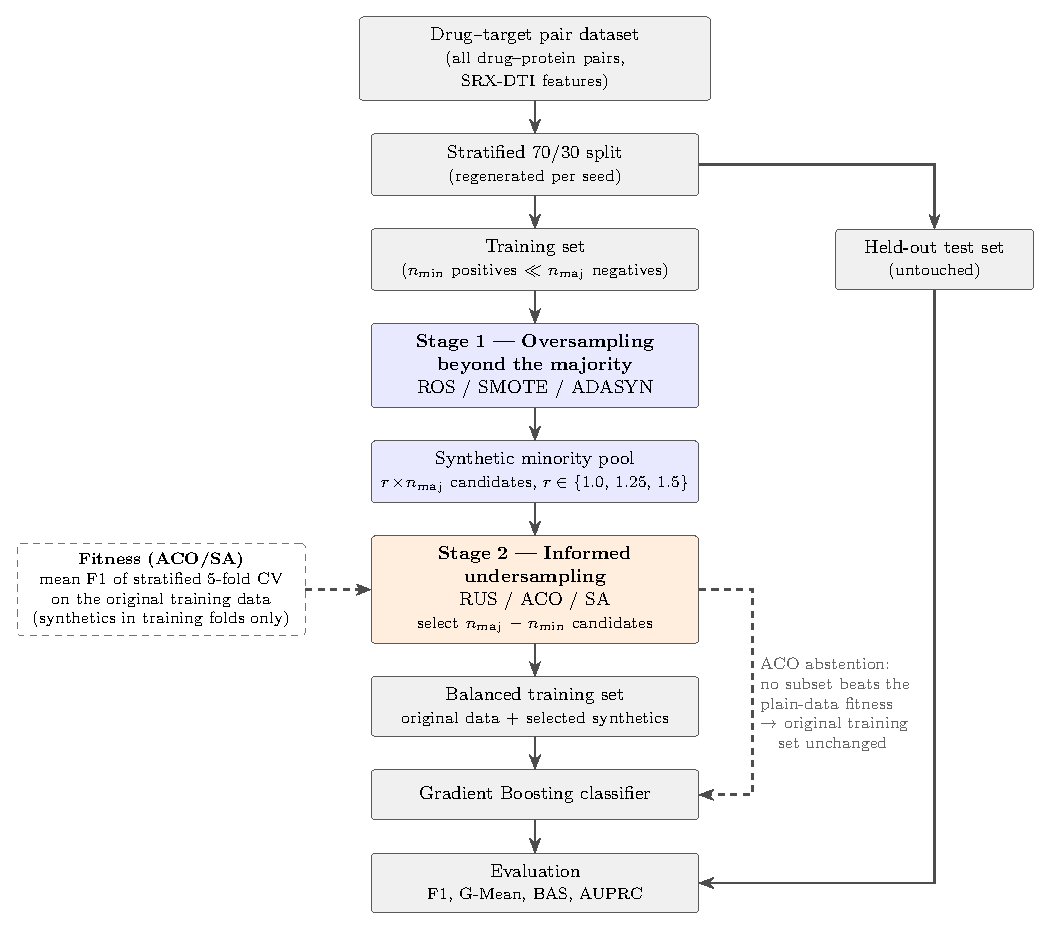
\includegraphics[width=0.78\textwidth]{F0_framework.pdf}
\caption{The workflow of the sequential hybrid sampling framework.}
\label{fig:framework}
\end{figure}

\subsection{ACO undersampler}
% [Draf narasi — menunggu validasi penulis]
The ACO undersampler searches for the subset of synthetic candidates that
maximizes a cross-validated fitness \citep{dorigo2006ant,
yu2013acosampling}. A solution is defined as a multiset of
$n_{\mathrm{maj}} - n_{\min}$ indices over the synthetic pool, so that
the union of the original training data and the selected candidates is
balanced. Each of the $K$ ants constructs a solution by sampling
candidate indices according to the selection probability expressed as
\begin{equation}
  P_i = \frac{\tau_i}{\sum_{j} \tau_j},
  \label{eq:prob}
\end{equation}
where $\tau_i$ denotes the pheromone value of candidate $i$. The
pheromone values were initialized uniformly at $\tau_0 = 0.3$. After all
ants finish in one iteration, the pheromone values were updated by using
the standard rule expressed as
\begin{equation}
  \tau_i^{(t+1)} = (1-\rho)\,\tau_i^{(t)} + \Delta_i,
  \label{eq:pheromone}
\end{equation}
where $\rho$ denotes the evaporation rate and $\Delta_i$ denotes the
fitness accumulated over the ants that selected candidate $i$. The
fitness of a solution was defined as the mean F1 score of a stratified
5-fold cross-validation on the original training data, in which the
selected synthetic candidates were added to the training folds only. The
search was run for $N = 10$ iterations with an early stop after five
iterations without improvement. The evaporation rate was set to
$\rho = 0.8$ following the tuning of the previous study, while the
number of ants $K$ is discussed in Section~\ref{sec:design}. The best
solution found across all iterations was returned as the final
selection. In addition, the implementation has an abstention property.
The fitness of the unmodified training data was evaluated as the initial
reference, and if no ant solution exceeds this reference, the
undersampler returns the original training data without any synthetic
candidates.

\subsubsection{Corrections to the previous implementation}
% [Draf narasi — menunggu validasi penulis]
We found three divergences between the implementation of the previous
study and the published equations. First, the pheromone update was
implemented as $\tau^{(t+1)} = (1-\rho\,\tau^{(t)}) + \Delta$ instead of
Eq.~(\ref{eq:pheromone}). Second, the cross-validation in the fitness
function was not stratified, so that a fold may contain no positive
instance under extreme imbalance. Third, the solution was constructed by
sampling with replacement, so that a solution may contain duplicated
candidates. We ablated the three factors in a full $2\times2\times2$
factorial design, and the results show that none of them significantly
affects the performance (Section~\ref{sec:ablation}). The final
configuration follows the published equations, i.e., the standard
pheromone update with stratified cross-validation, while the selection
with replacement was retained.

\subsection{Budget-matched SA comparator}
\begin{poin}
  \item Motivasi: memisahkan ``manfaat seleksi terinformasi'' dari
        ``manfaat ACO spesifik'' \citep{chennuru2022simulated}.
  \item SA klasik \citep{kirkpatrick1983optimization}: satu solusi
        berjalan; tetangga = resample 5\% posisi; penerimaan Boltzmann
        $\exp(\Delta/T)$.
  \item Cooling geometrik $T$: 0,05 $\rightarrow$ 0,001 sepanjang budget.
  \item Budget evaluasi fitness = $K \times N$ milik ACO (identik); fungsi
        fitness \& ruang solusi identik.
  \item Klaim fairness: satu-satunya perbedaan = strategi pencarian.
\end{poin}

\subsection{Compared methods}
\begin{poin}
  \item 13 metode per dataset: baseline GB; ROS/SMOTE/ADASYN klasik;
        SMOTE-ENN, SMOTE-Tomek \citep{batista2004study}; SHS-RUS $\times$3;
        SHS-ACO $\times$3; SHS-SA (SMOTE).
  \item Classifier seragam: Gradient Boosting \citep{friedman2001greedy}.
  \item Alasan tidak menambah classifier lain: isolasi efek sampling.
\end{poin}

\subsection{Experimental design}
\label{sec:design}
\begin{poin}
  \item P0 reproduksi: konfigurasi persis paper 1, 5 seed.
  \item P0b ekuivalensi GB vs HistGB (10 seed berpasangan).
  \item P1 ablasi $2\times2\times2$ koreksi ACO + fitness \{F1, G-Mean,
        BAS\} (NR, 5 seed, Wilcoxon berpasangan).
  \item P2 pilot rasio \{1,0; 1,25; 1,5\} $\times$ 6 metode SHS (NR).
  \item P2b sensitivitas $\rho$ \{0,5; 0,95\}, $K$ \{10; 40\} + duel SA.
  \item P3 perbandingan penuh 13 metode $\times$ 4 dataset; seed 0--9
        metode murah, 0--4 ACO/SA.
  \item Split stratified 70/30 per seed; sampling hanya pada train; seed
        identik antar metode (berpasangan).
  \item Keputusan berbasis pilot: $K$=10 (setara $K$=20 pada separuh
        biaya); rasio per lengan (RUS 1,25/1,25/1,0; ACO/SA 1,5).
  \item Enzyme: fitness internal memakai HistGB \citep{ke2017lightgbm}
        (fit GB 810\,s vs HistGB 82,7\,s); classifier final tetap GB;
        seragam dalam dataset.
  \item Kompute: server cloud 12 vCPU; \texttt{OMP\_NUM\_THREADS}=1; job
        per-seed paralel.
\end{poin}

\subsection{Metrics and statistical tests}
\begin{poin}
  \item Metrik: F1 (primer), G-Mean, BAS \citep{cahyana2019improving};
        + AUPRC (threshold-free) \citep{saito2015precision}.
  \item Semua dari confusion matrix pada test set tak tersentuh.
  \item Per dataset: Wilcoxon signed-rank berpasangan (seed sama),
        $\alpha$=0,05.
  \item Lintas dataset: Friedman + post-hoc Nemenyi pada blok
        dataset$\times$seed, mean ranks \citep{demsar2006statistical}.
  \item Runtime dilaporkan per metode (mesin sama, disclaimer paralelisme).
\end{poin}

\subsection{Implementation and reproducibility}
\begin{poin}
  \item Python 3.12; scikit-learn \citep{pedregosa2011scikit},
        imbalanced-learn \citep{lemaitre2017imbalanced}.
  \item Semua run ber-seed penuh $\rightarrow$ deterministik (baris identik
        lintas mesin/waktu).
  \item Kode, pipeline data, seluruh CSV hasil: repositori publik
        (\url{https://github.com/ismankrn/aco-shs}; buat rilis/tag saat
        submit).
\end{poin}

% =========================================================================
\section{Results}

\subsection{Reproduction and seed sensitivity}
\begin{poin}
  \item Konfigurasi paper 1: F1 = $0{,}3606 \pm 0{,}0707$ (5 seed), rentang
        0,2667--0,4314 (Tabel~\ref{tab:repro}).
  \item 2/5 seed tepat di 0,4314 $\approx$ angka publikasi 0,4324
        $\rightarrow$ tereproduksi, tapi ujung optimis.
  \item 1 TP $\approx$ 4,3 poin recall di NR (27 positif test)
        $\rightarrow$ argumen protokol berulang.
\end{poin}

\begin{table}[htbp]
\centering
\caption{\todocap{reproduksi konfigurasi tesis per seed; referensi split
tunggal F1=0,4324}}
\label{tab:repro}
\begin{tabular}{lcccc}
\toprule
Seed & F1 & G-Mean & BAS & AUPRC \\
\midrule
0 & 0.2667 & 0.4642 & 0.5959 & 0.2713 \\
1 & 0.4314 & 0.6277 & 0.6872 & 0.3764 \\
2 & 0.4314 & 0.6277 & 0.6872 & 0.3449 \\
3 & 0.3333 & 0.5040 & 0.6195 & 0.3239 \\
4 & 0.3404 & 0.5360 & 0.6330 & 0.3144 \\
\midrule
Mean $\pm$ SD & 0.3606 $\pm$ 0.0707 & 0.5519 $\pm$ 0.0737 & 0.6446 $\pm$ 0.0411 & 0.3262 $\pm$ 0.0388 \\
\bottomrule
\end{tabular}

\end{table}

\subsection{ACO ablation and sensitivity}
\label{sec:ablation}
\begin{poin}
  \item Per faktor ($n$=20 pasangan): legacy $p$=0,925; stratified
        $p$=0,554; replacement $p$=0,112 (Tabel~\ref{tab:ablation}).
  \item Refined vs thesis-like: $p$=1,0 $\rightarrow$ koreksi tidak
        mengubah hasil (robustness).
  \item Fitness: F1 0,3381 $\approx$ G-Mean 0,3389; BAS lebih buruk 0,3081.
  \item $\rho$ \{0,5--0,95\} \& $K$ \{10--40\} tak signifikan; $K$=10 =
        kualitas $K$=20 pada separuh biaya (Tabel~\ref{tab:sensitivity}).
  \item Dari log konvergensi: fitness mendatar di iterasi $\sim$6--8
        $\rightarrow$ $N$=10 cukup (Gambar~\ref{fig:convergence}).
\end{poin}

\begin{table}[htbp]
\centering
\caption{\todocap{ablasi 2$\times$2$\times$2 + fungsi fitness; variant A/B =
False/True per faktor}}
\label{tab:ablation}
\resizebox{\textwidth}{!}{\begin{tabular}{lcccc}
\toprule
Comparison & F1 (A) & F1 (B) & $n$ & $p$ (Wilcoxon) \\
\midrule
Pheromone update (standard vs multiplicative) & 0.3338 & 0.3347 & 20 & 0.9246 \\
Fitness CV (plain vs stratified) & 0.3368 & 0.3317 & 20 & 0.5540 \\
Selection (w/o vs with replacement) & 0.3244 & 0.3441 & 20 & 0.1119 \\
Default vs alternative configuration & 0.3381 & 0.3410 & 5 & 1.0000 \\
\midrule
Fitness function = F1 & 0.3381 & -- & 5 & -- \\
Fitness function = GMEAN & 0.3389 & -- & 5 & -- \\
Fitness function = BAS & 0.3081 & -- & 5 & -- \\
\bottomrule
\end{tabular}
}
\end{table}

\begin{table}[htbp]
\centering
\caption{\todocap{sensitivitas $\rho$/$K$ + SA budget-matched; NR,
SHS-ACO-SMOTE rasio 1,5}}
\label{tab:sensitivity}
\begin{tabular}{lccc}
\toprule
Variant & F1 (mean $\pm$ SD) & $p$ vs default & Runtime/seed \\
\midrule
Default ($\rho$=0.8, $K$=20) & 0.3431 $\pm$ 0.0936 & -- & 1.9\,h \\
$\rho$ = 0.5 & 0.3461 $\pm$ 0.0819 & 1.0000 & 1.8\,h \\
$\rho$ = 0.95 & 0.3590 $\pm$ 0.0722 & 0.6250 & 1.8\,h \\
$K$ = 10 & 0.3507 $\pm$ 0.1037 & 1.0000 & 52.5\,min \\
$K$ = 40 & 0.3223 $\pm$ 0.0839 & 0.3125 & 3.3\,h \\
SA (budget-matched) & 0.3565 $\pm$ 0.0676 & 0.6250 & 2.0\,h \\
\bottomrule
\end{tabular}

\end{table}

\subsection{Pool ratio $\times$ selector interaction}
\begin{poin}
  \item ACO terbaik selalu di rasio 1,5 (ketiga oversampler); RUS terbaik
        di 1,0--1,25 (Tabel~\ref{tab:ratio}, Gambar~\ref{fig:ratio}).
  \item Interpretasi mekanistik: surplus = ruang pilihan bagi selektor
        terinformasi, noise bagi selektor acak.
\end{poin}

\begin{table}[htbp]
\centering
\caption{\todocap{F1 per rasio pool (NR, 5 seed); tebal = rasio terbaik per
metode}}
\label{tab:ratio}
\resizebox{\textwidth}{!}{\begin{tabular}{lccc}
\toprule
Method & Ratio 1.00 & Ratio 1.25 & Ratio 1.50 \\
\midrule
SHS-RUS (ROS) & 0.4579 $\pm$ 0.0531 & \textbf{0.4725 $\pm$ 0.0611} & 0.4586 $\pm$ 0.0551 \\
SHS-RUS (SMOTE) & 0.3735 $\pm$ 0.0888 & \textbf{0.3759 $\pm$ 0.0856} & 0.3419 $\pm$ 0.0721 \\
SHS-RUS (ADASYN) & \textbf{0.3805 $\pm$ 0.0918} & 0.3665 $\pm$ 0.0899 & 0.3187 $\pm$ 0.0852 \\
SHS-ACO (ROS) & 0.4736 $\pm$ 0.0680 & 0.4390 $\pm$ 0.0518 & \textbf{0.4751 $\pm$ 0.0739} \\
SHS-ACO (SMOTE) & 0.3130 $\pm$ 0.0772 & 0.3381 $\pm$ 0.0675 & \textbf{0.3431 $\pm$ 0.0936} \\
SHS-ACO (ADASYN) & 0.3451 $\pm$ 0.0822 & 0.3276 $\pm$ 0.1264 & \textbf{0.3603 $\pm$ 0.1094} \\
\bottomrule
\end{tabular}
}
\end{table}

\begin{figure}[htbp]
\centering
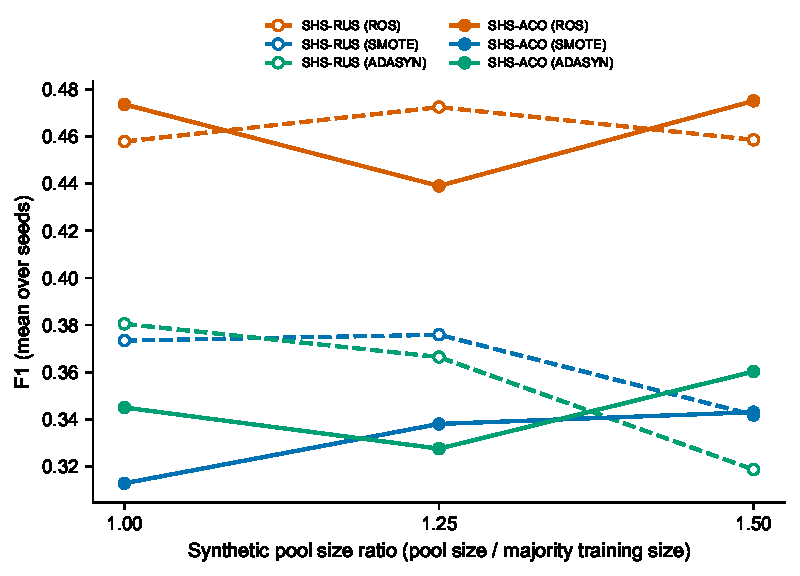
\includegraphics[width=0.75\textwidth]{F2_ratio_interaction.pdf}
\caption{\todocap{solid = SHS-ACO, putus-putus = SHS-RUS; warna = arm
oversampler; ACO naik dengan ukuran pool, RUS sebaliknya}}
\label{fig:ratio}
\end{figure}

\subsection{Main comparison across four datasets}
\begin{poin}
  \item Tabel inti: Tabel~\ref{tab:main} (G-Mean/BAS/AUPRC di suplemen).
  \item NR: keluarga ROS dominan (RUS-ROS 0,473) $\gg$ SMOTE; GPCR: ROS
        runtuh, SHS-SA-SMOTE 0,365 memimpin tipis atas SMOTE-Tomek 0,361;
        IC: SHS-ACO-ADASYN 0,346; Enzyme: baseline 0,185 tak terkalahkan.
  \item Tidak ada juara universal; juara oversampler bergeser
        ROS $\rightarrow$ SMOTE $\rightarrow$ ADASYN $\rightarrow$ tanpa
        sampling mengikuti kekayaan positif asli
        (Gambar~\ref{fig:gradient}).
  \item Uji per dataset: Tabel~\ref{tab:tests}; $n$=5 memberi $p$ minimum
        0,0625 (GPCR/IC mencapainya).
  \item Friedman $\chi^2$=42,5, $p$=2,7$\times10^{-5}$; rank teratas
        SHS-ACO-ADASYN 4,85 dan SHS-ACO-SMOTE 5,00; CD Nemenyi = 4,08:
        hanya baseline/ROS/SHS-RUS-ROS terpisah dari yang terbaik
        (Gambar~\ref{fig:ranks}).
\end{poin}

\begin{table}[htbp]
\centering
\caption{\todocap{tabel inti F1 mean$\pm$SD, 13 metode $\times$ 4 dataset;
tebal = terbaik per dataset}}
\label{tab:main}
\resizebox{\textwidth}{!}{\begin{tabular}{lccccc}
\toprule
Method & $n$ & NR & GPCR & IC & Enzyme \\
\midrule
Baseline (no resampling) & 10 & 0.3235 $\pm$ 0.0870 & 0.1925 $\pm$ 0.0388 & 0.1600 $\pm$ 0.0246 & \textbf{0.1854 $\pm$ 0.0158} \\
ROS & 10 & 0.4573 $\pm$ 0.0537 & 0.2404 $\pm$ 0.0098 & 0.2621 $\pm$ 0.0065 & 0.1137 $\pm$ 0.0019 \\
SMOTE & 10 & 0.3744 $\pm$ 0.0900 & 0.3582 $\pm$ 0.0371 & 0.3221 $\pm$ 0.0131 & 0.1726 $\pm$ 0.0067 \\
ADASYN & 10 & 0.3582 $\pm$ 0.1025 & 0.3098 $\pm$ 0.0405 & 0.3412 $\pm$ 0.0160 & 0.1489 $\pm$ 0.0049 \\
SMOTE-ENN & 10 & 0.3469 $\pm$ 0.0467 & 0.3184 $\pm$ 0.0216 & 0.3032 $\pm$ 0.0133 & 0.1726 $\pm$ 0.0076 \\
SMOTE-Tomek & 10 & 0.3890 $\pm$ 0.0815 & 0.3614 $\pm$ 0.0337 & 0.3203 $\pm$ 0.0139 & 0.1728 $\pm$ 0.0067 \\
SHS-RUS (ROS) & 10 & \textbf{0.4725 $\pm$ 0.0611} & 0.2393 $\pm$ 0.0090 & 0.2635 $\pm$ 0.0070 & 0.1137 $\pm$ 0.0026 \\
SHS-RUS (SMOTE) & 10 & 0.3759 $\pm$ 0.0856 & 0.3440 $\pm$ 0.0407 & 0.3206 $\pm$ 0.0144 & 0.1743 $\pm$ 0.0053 \\
SHS-RUS (ADASYN) & 10 & 0.3805 $\pm$ 0.0918 & 0.3199 $\pm$ 0.0417 & 0.3444 $\pm$ 0.0196 & 0.1512 $\pm$ 0.0047 \\
SHS-ACO (ROS) & 5 & 0.4338 $\pm$ 0.0619 & 0.2370 $\pm$ 0.0086 & 0.2684 $\pm$ 0.0080 & 0.1840 $\pm$ 0.0106 \\
SHS-ACO (SMOTE) & 5 & 0.3507 $\pm$ 0.1037 & 0.3516 $\pm$ 0.0596 & 0.3246 $\pm$ 0.0184 & 0.1840 $\pm$ 0.0106 \\
SHS-ACO (ADASYN) & 5 & 0.3930 $\pm$ 0.0889 & 0.2890 $\pm$ 0.0519 & \textbf{0.3461 $\pm$ 0.0224} & 0.1840 $\pm$ 0.0106 \\
SHS-SA (SMOTE) & 5 & 0.3467 $\pm$ 0.0738 & \textbf{0.3645 $\pm$ 0.0554} & 0.3205 $\pm$ 0.0148 & 0.1707 $\pm$ 0.0034 \\
\bottomrule
\end{tabular}
}
\end{table}

\begin{table}[htbp]
\centering
\caption{\todocap{pemenang per dataset + Wilcoxon berpasangan; '--' Enzyme =
skor identik karena abstensi}}
\label{tab:tests}
\resizebox{\textwidth}{!}{\begin{tabular}{lcccccc}
\toprule
Dataset & Best method & F1 & Runner-up & $p$ (vs runner-up) & F1 baseline & $p$ (vs baseline) \\
\midrule
NR & SHS-RUS (ROS) & 0.4725 & ROS & 0.8203 & 0.3235 & 0.0059 \\
GPCR & SHS-SA (SMOTE) & 0.3645 & SMOTE-Tomek & 0.6250 & 0.1925 & 0.0625 \\
IC & SHS-ACO (ADASYN) & 0.3461 & SHS-RUS (ADASYN) & 0.4375 & 0.1600 & 0.0625 \\
Enzyme & Baseline (no resampling) & 0.1854 & SHS-ACO (ADASYN) & -- & 0.1854 & -- \\
\bottomrule
\end{tabular}
}
\end{table}

\begin{figure}[htbp]
\centering
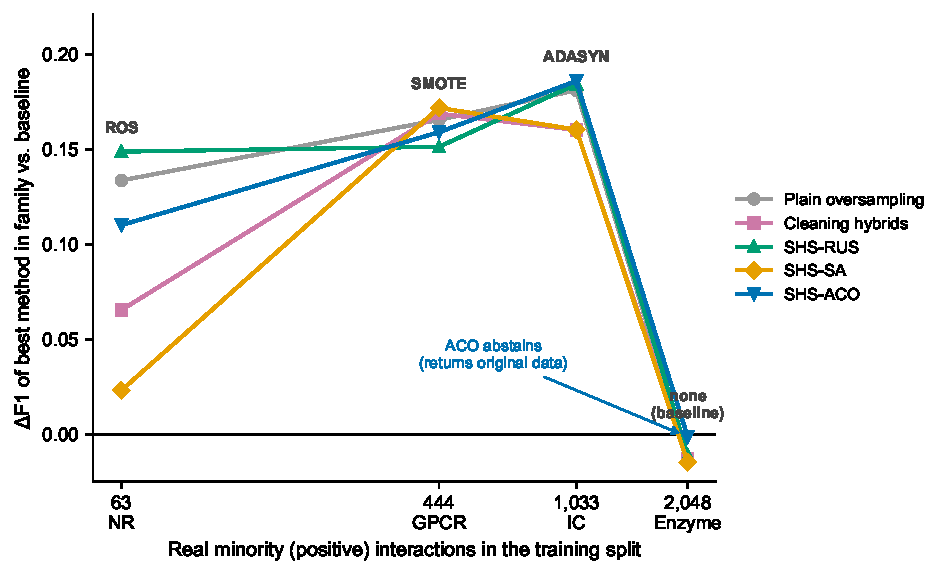
\includegraphics[width=0.9\textwidth]{F1_gradient.pdf}
\caption{\todocap{$\Delta$F1 metode terbaik per keluarga vs baseline; sumbu-x
log positif asli train; label atas = oversampler juara; titik ACO-Enzyme =
abstensi}}
\label{fig:gradient}
\end{figure}

\begin{figure}[htbp]
\centering
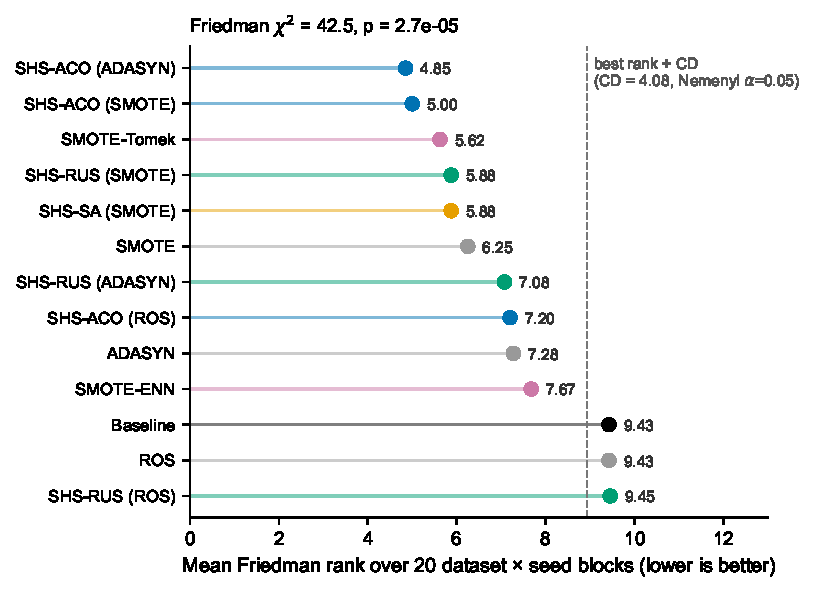
\includegraphics[width=0.8\textwidth]{F4_friedman_ranks.pdf}
\caption{\todocap{mean rank Friedman 20 blok; garis putus = best + CD
Nemenyi $\alpha$=0,05; kiri garis = tak terbedakan dari terbaik}}
\label{fig:ranks}
\end{figure}

\subsection{The ACO abstention property}
\begin{poin}
  \item Di Enzyme, fitness ACO tak pernah menemukan subset sintetis yang
        mengalahkan data asli $\rightarrow$ fallback mengembalikan data
        latih asli di 15/15 run (Tabel~\ref{tab:abstention}).
  \item Verifikasi: confusion matrix identik dengan baseline di semua
        15 run (3 arm $\times$ 5 seed).
  \item SA tanpa opsi abstain terpaksa oversampling $\rightarrow$ sedikit
        di bawah baseline (0,171 vs 0,185).
  \item Interpretasi: seleksi terinformasi + aksi-nol = katup pengaman;
        rekomendasi desain eksplisit.
\end{poin}

\begin{table}[htbp]
\centering
\caption{\todocap{verifikasi abstensi per seed di Enzyme; 'identical' =
confusion matrix sama dengan baseline}}
\label{tab:abstention}
\resizebox{\textwidth}{!}{\begin{tabular}{lccccc}
\toprule
Seed & F1 baseline & ACO (ROS) & ACO (SMOTE) & ACO (ADASYN) & F1 SHS-SA (SMOTE) \\
\midrule
0 & 0.1889 & identical & identical & identical & 0.1684 \\
1 & 0.1711 & identical & identical & identical & 0.1716 \\
2 & 0.1980 & identical & identical & identical & 0.1690 \\
3 & 0.1860 & identical & identical & identical & 0.1762 \\
4 & 0.1761 & identical & identical & identical & 0.1682 \\
\bottomrule
\end{tabular}
}
\end{table}

\subsection{ACO versus SA}
\begin{poin}
  \item Tak signifikan di semua dataset ($p$ 0,125--0,812;
        Tabel~\ref{tab:savsaco}); SA menang GPCR nominal, ACO menang
        IC/Enzyme nominal.
  \item Konvergensi budget-matched: keduanya melompat di $\sim$20 evaluasi
        pertama lalu mendatar; akhir 0,601 vs 0,595
        (Gambar~\ref{fig:convergence}).
  \item Kesimpulan: pilihan metaheuristik sekunder; asimetri abstensi yang
        membedakan desain ACO.
\end{poin}

\begin{table}[htbp]
\centering
\caption{\todocap{SA vs ACO per dataset, arm SMOTE, seed berpasangan}}
\label{tab:savsaco}
\resizebox{\textwidth}{!}{\begin{tabular}{lccccc}
\toprule
Dataset & F1 SHS-ACO (SMOTE) & F1 SHS-SA (SMOTE) & Diff. & $n$ & $p$ (Wilcoxon) \\
\midrule
NR & 0.3507 & 0.3467 & +0.0039 & 5 & 0.8125 \\
GPCR & 0.3516 & 0.3645 & -0.0128 & 5 & 0.3750 \\
IC & 0.3246 & 0.3205 & +0.0042 & 5 & 0.6250 \\
Enzyme & 0.1840 & 0.1707 & +0.0133 & 5 & 0.1250 \\
\bottomrule
\end{tabular}
}
\end{table}

\begin{figure}[htbp]
\centering
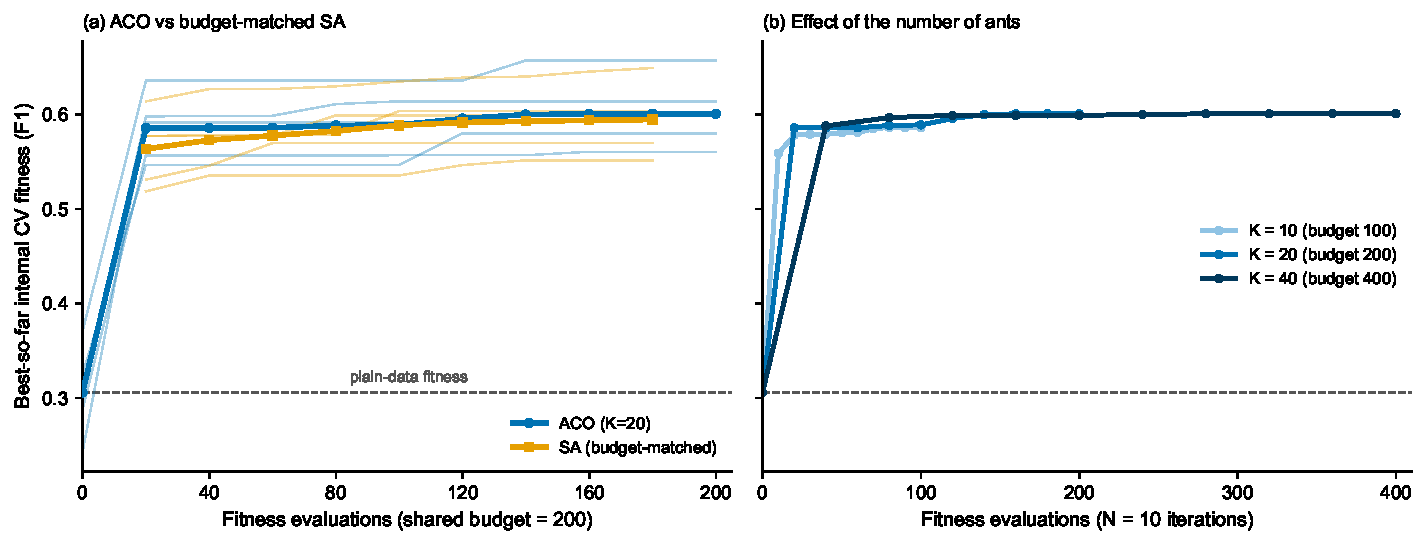
\includegraphics[width=0.75\textwidth]{F3_convergence.pdf}
\caption{\todocap{best-so-far fitness CV internal vs evaluasi, NR budget 200;
garis tipis = seed; garis putus = fitness data asli (ambang abstensi)}}
\label{fig:convergence}
\end{figure}

\subsection{Computational cost}
\begin{poin}
  \item RUS/hybrid murah 2\,s--2,5\,min/seed vs ACO/SA
        22\,min--20\,h/seed: 500--1.700$\times$ (Tabel~\ref{tab:runtime}).
  \item SA $\approx$ ACO (budget sama); $K$=10 separuh biaya $K$=20.
  \item Sandingkan dengan $\Delta$F1 tipis $\rightarrow$ kerangka keputusan
        biaya-manfaat di Discussion.
\end{poin}

\begin{table}[htbp]
\centering
\caption{\todocap{runtime per seed (sampling + training final), relatif thd
baseline; mesin identik}}
\label{tab:runtime}
\resizebox{\textwidth}{!}{\begin{tabular}{lrrrr}
\toprule
Method & NR & GPCR & IC & Enzyme \\
\midrule
Baseline (no resampling) & 2.1\,s (1$\times$) & 39.1\,s (1$\times$) & 1.6\,min (1$\times$) & 13.0\,min (1$\times$) \\
ROS & 3.4\,s (2$\times$) & 1.2\,min (2$\times$) & 2.9\,min (2$\times$) & 25.0\,min (2$\times$) \\
SMOTE & 7.6\,s (4$\times$) & 2.2\,min (3$\times$) & 6.8\,min (4$\times$) & 1.0\,h (5$\times$) \\
ADASYN & 7.1\,s (3$\times$) & 2.1\,min (3$\times$) & 6.2\,min (4$\times$) & 57.0\,min (4$\times$) \\
SMOTE-ENN & 7.3\,s (3$\times$) & 2.5\,min (4$\times$) & 8.3\,min (5$\times$) & 1.2\,h (6$\times$) \\
SMOTE-Tomek & 7.7\,s (4$\times$) & 2.6\,min (4$\times$) & 8.5\,min (5$\times$) & 1.2\,h (5$\times$) \\
SHS-RUS (ROS) & 3.5\,s (2$\times$) & 1.2\,min (2$\times$) & 2.9\,min (2$\times$) & 25.2\,min (2$\times$) \\
SHS-RUS (SMOTE) & 7.8\,s (4$\times$) & 2.2\,min (3$\times$) & 6.9\,min (4$\times$) & 1.0\,h (5$\times$) \\
SHS-RUS (ADASYN) & 6.9\,s (3$\times$) & 2.1\,min (3$\times$) & 6.2\,min (4$\times$) & 58.8\,min (5$\times$) \\
SHS-ACO (ROS) & 22.5\,min (635$\times$) & 8.6\,h (790$\times$) & 20.8\,h (779$\times$) & 11.2\,h (52$\times$) \\
SHS-ACO (SMOTE) & 49.4\,min (1394$\times$) & 15.4\,h (1419$\times$) & 45.1\,h (1691$\times$) & 12.1\,h (56$\times$) \\
SHS-ACO (ADASYN) & 48.2\,min (1360$\times$) & 13.3\,h (1225$\times$) & 43.2\,h (1621$\times$) & 12.3\,h (57$\times$) \\
SHS-SA (SMOTE) & 58.0\,min (1634$\times$) & 17.2\,h (1583$\times$) & 51.5\,h (1930$\times$) & 12.9\,h (60$\times$) \\
\bottomrule
\end{tabular}
}
\end{table}

% =========================================================================
\section{Discussion}
\begin{poin}
  \item Temuan payung: evaluasi split-tunggal menyesatkan — kesimpulan
        paper 1 (SMOTE+ACO juara) tidak bertahan di bawah protokol
        berulang maupun lintas dataset.
  \item ``Ceiling hypothesis'': karakter oversampler $\times$ dataset
        menentukan langit-langit; selektor menentukan seberapa dekat ke
        langit-langit.
  \item Manfaat seleksi terinformasi menyusut saat positif asli cukup
        banyak (selisih selektor: $+0{,}015 \rightarrow +0{,}006
        \rightarrow +0{,}005 \rightarrow$ abstain); hipotesis: kualitas
        sintetis lebih seragam $\rightarrow$ memilih tidak menambah nilai.
  \item Catatan jujur: $\Delta$F1 keluarga thd baseline bertahan
        0,13--0,19 sampai IC lalu \emph{runtuh} di Enzyme (bukan penurunan
        monoton) — yang monoton adalah selisih seleksi dan pergeseran
        juara.
  \item ACO vs SA setara $\rightarrow$ jawaban langsung ``mengapa ACO'';
        yang membedakan adalah aksi abstain, bukan pencariannya
        \citep{kirkpatrick1983optimization, chennuru2022simulated}.
  \item Robustness menyeluruh (aturan, parameter, optimizer) = kabar baik
        praktisi; koreksi kode-vs-persamaan dilaporkan sebagai praktik
        transparansi.
  \item Trade-off biaya: kapan 15 jam komputasi layak untuk $\leq$1 poin
        F1? — kerangka keputusan untuk pembaca.
  \item Threats to validity: asumsi negatif; 5 seed untuk lengan mahal
        ($p$ minimum 0,0625); HistGB fitness khusus Enzyme; satu
        classifier; satu domain (DTI).
  \item Future work: classifier lain, dataset non-DTI, surrogate fitness
        murah, GA/PSO (disebut, tidak diuji).
\end{poin}

% =========================================================================
\section{Conclusions}
\begin{poin}
  \item SHS valid tetapi kondisional — peta kapan-apa (dataset
        kecil/ekstrem: ya; besar: oversampler sederhana cukup; sangat
        kaya: jangan sampling, dan ACO tahu kapan tidak).
  \item Seleksi terinformasi $>$ acak pada kondisi yang tepat;
        metaheuristiknya bebas dipilih.
  \item Protokol evaluasi berulang + statistik = rekomendasi baku untuk
        riset sampling-DTI ke depan.
  \item Kode/data terbuka.
\end{poin}

% =========================================================================
\section*{Acknowledgements}
% TODO: dana/fasilitas (mis. Telkom University), bantuan komputasi.

\section*{Data Availability}
% Poin: kode + CSV hasil + skrip regenerasi fitur di
% https://github.com/ismankrn/aco-shs (buat tag/rilis + DOI Zenodo saat
% submit); fitur sumber dari repo SRX-DTI [khojasteh2023improving].

\section*{Author Contributions}
% RNH: eksperimen awal (paper 1), kurasi data, draf.
% IK: konseptualisasi, supervisi, validasi, penulisan — review & editing,
%     corresponding author. (Sesuaikan dengan CRediT.)

\bibliographystyle{unsrtnat}
\bibliography{references}

% =========================================================================
\appendix
\section{Supplemental tables}
% Pindahkan ke file suplemen terpisah saat submission PeerJ.

\begin{table}[htbp]
\centering
\caption{G-Mean (mean $\pm$ SD), 13 methods $\times$ 4 datasets.}
\resizebox{\textwidth}{!}{\begin{tabular}{lccccc}
\toprule
Method & $n$ & NR & GPCR & IC & Enzyme \\
\midrule
Baseline (no resampling) & 10 & 0.4709 $\pm$ 0.0754 & 0.3332 $\pm$ 0.0386 & 0.3004 $\pm$ 0.0260 & 0.3272 $\pm$ 0.0149 \\
ROS & 10 & 0.7296 $\pm$ 0.0490 & 0.7925 $\pm$ 0.0131 & 0.8265 $\pm$ 0.0076 & \textbf{0.8456 $\pm$ 0.0071} \\
SMOTE & 10 & 0.5498 $\pm$ 0.0733 & 0.5511 $\pm$ 0.0367 & 0.6519 $\pm$ 0.0121 & 0.6554 $\pm$ 0.0150 \\
ADASYN & 10 & 0.5438 $\pm$ 0.0855 & 0.5054 $\pm$ 0.0404 & 0.6560 $\pm$ 0.0164 & 0.6402 $\pm$ 0.0119 \\
SMOTE-ENN & 10 & 0.6364 $\pm$ 0.0525 & 0.6879 $\pm$ 0.0212 & 0.7080 $\pm$ 0.0143 & 0.6612 $\pm$ 0.0217 \\
SMOTE-Tomek & 10 & 0.5609 $\pm$ 0.0632 & 0.5527 $\pm$ 0.0343 & 0.6473 $\pm$ 0.0148 & 0.6551 $\pm$ 0.0150 \\
SHS-RUS (ROS) & 10 & \textbf{0.7358 $\pm$ 0.0503} & \textbf{0.7933 $\pm$ 0.0141} & 0.8286 $\pm$ 0.0085 & 0.8449 $\pm$ 0.0081 \\
SHS-RUS (SMOTE) & 10 & 0.5442 $\pm$ 0.0693 & 0.5314 $\pm$ 0.0359 & 0.6451 $\pm$ 0.0122 & 0.6579 $\pm$ 0.0138 \\
SHS-RUS (ADASYN) & 10 & 0.5621 $\pm$ 0.0720 & 0.5130 $\pm$ 0.0415 & 0.6561 $\pm$ 0.0201 & 0.6449 $\pm$ 0.0158 \\
SHS-ACO (ROS) & 5 & 0.7134 $\pm$ 0.0581 & 0.7898 $\pm$ 0.0100 & \textbf{0.8296 $\pm$ 0.0096} & 0.3260 $\pm$ 0.0095 \\
SHS-ACO (SMOTE) & 5 & 0.5382 $\pm$ 0.0820 & 0.5478 $\pm$ 0.0575 & 0.6525 $\pm$ 0.0210 & 0.3260 $\pm$ 0.0095 \\
SHS-ACO (ADASYN) & 5 & 0.5837 $\pm$ 0.0729 & 0.4872 $\pm$ 0.0541 & 0.6684 $\pm$ 0.0196 & 0.3260 $\pm$ 0.0095 \\
SHS-SA (SMOTE) & 5 & 0.5344 $\pm$ 0.0548 & 0.5581 $\pm$ 0.0576 & 0.6458 $\pm$ 0.0165 & 0.6474 $\pm$ 0.0059 \\
\bottomrule
\end{tabular}
}
\end{table}

\begin{table}[htbp]
\centering
\caption{Balanced accuracy (mean $\pm$ SD), 13 methods $\times$ 4 datasets.}
\resizebox{\textwidth}{!}{\begin{tabular}{lccccc}
\toprule
Method & $n$ & NR & GPCR & IC & Enzyme \\
\midrule
Baseline (no resampling) & 10 & 0.6087 $\pm$ 0.0359 & 0.5555 $\pm$ 0.0124 & 0.5447 $\pm$ 0.0079 & 0.5534 $\pm$ 0.0048 \\
ROS & 10 & 0.7537 $\pm$ 0.0390 & 0.7957 $\pm$ 0.0120 & 0.8267 $\pm$ 0.0075 & \textbf{0.8461 $\pm$ 0.0069} \\
SMOTE & 10 & 0.6449 $\pm$ 0.0424 & 0.6481 $\pm$ 0.0203 & 0.6995 $\pm$ 0.0084 & 0.7046 $\pm$ 0.0100 \\
ADASYN & 10 & 0.6413 $\pm$ 0.0498 & 0.6237 $\pm$ 0.0208 & 0.7036 $\pm$ 0.0110 & 0.6926 $\pm$ 0.0079 \\
SMOTE-ENN & 10 & 0.6829 $\pm$ 0.0365 & 0.7241 $\pm$ 0.0155 & 0.7341 $\pm$ 0.0111 & 0.7084 $\pm$ 0.0144 \\
SMOTE-Tomek & 10 & 0.6509 $\pm$ 0.0379 & 0.6490 $\pm$ 0.0189 & 0.6965 $\pm$ 0.0101 & 0.7044 $\pm$ 0.0101 \\
SHS-RUS (ROS) & 10 & \textbf{0.7591 $\pm$ 0.0401} & \textbf{0.7964 $\pm$ 0.0126} & 0.8288 $\pm$ 0.0082 & 0.8454 $\pm$ 0.0078 \\
SHS-RUS (SMOTE) & 10 & 0.6423 $\pm$ 0.0401 & 0.6376 $\pm$ 0.0193 & 0.6952 $\pm$ 0.0085 & 0.7063 $\pm$ 0.0092 \\
SHS-RUS (ADASYN) & 10 & 0.6510 $\pm$ 0.0425 & 0.6278 $\pm$ 0.0210 & 0.7040 $\pm$ 0.0135 & 0.6958 $\pm$ 0.0105 \\
SHS-ACO (ROS) & 5 & 0.7407 $\pm$ 0.0450 & 0.7930 $\pm$ 0.0093 & \textbf{0.8299 $\pm$ 0.0094} & 0.5529 $\pm$ 0.0031 \\
SHS-ACO (SMOTE) & 5 & 0.6369 $\pm$ 0.0491 & 0.6468 $\pm$ 0.0316 & 0.7001 $\pm$ 0.0145 & 0.5529 $\pm$ 0.0031 \\
SHS-ACO (ADASYN) & 5 & 0.6626 $\pm$ 0.0479 & 0.6148 $\pm$ 0.0268 & 0.7118 $\pm$ 0.0140 & 0.5529 $\pm$ 0.0031 \\
SHS-SA (SMOTE) & 5 & 0.6337 $\pm$ 0.0320 & 0.6527 $\pm$ 0.0312 & 0.6957 $\pm$ 0.0112 & 0.6992 $\pm$ 0.0036 \\
\bottomrule
\end{tabular}
}
\end{table}

\begin{table}[htbp]
\centering
\caption{AUPRC (mean $\pm$ SD), 13 methods $\times$ 4 datasets.}
\resizebox{\textwidth}{!}{\begin{tabular}{lccccc}
\toprule
Method & $n$ & NR & GPCR & IC & Enzyme \\
\midrule
Baseline (no resampling) & 10 & 0.4015 $\pm$ 0.0816 & \textbf{0.3439 $\pm$ 0.0300} & \textbf{0.4081 $\pm$ 0.0337} & \textbf{0.3191 $\pm$ 0.0131} \\
ROS & 10 & 0.4038 $\pm$ 0.0720 & 0.3091 $\pm$ 0.0323 & 0.3636 $\pm$ 0.0289 & 0.1643 $\pm$ 0.0092 \\
SMOTE & 10 & 0.3665 $\pm$ 0.0816 & 0.3241 $\pm$ 0.0333 & 0.2663 $\pm$ 0.0307 & 0.0958 $\pm$ 0.0055 \\
ADASYN & 10 & 0.3400 $\pm$ 0.0625 & 0.2829 $\pm$ 0.0261 & 0.2511 $\pm$ 0.0235 & 0.0816 $\pm$ 0.0035 \\
SMOTE-ENN & 10 & 0.2739 $\pm$ 0.0505 & 0.2884 $\pm$ 0.0272 & 0.2513 $\pm$ 0.0188 & 0.0967 $\pm$ 0.0066 \\
SMOTE-Tomek & 10 & 0.3645 $\pm$ 0.0847 & 0.3242 $\pm$ 0.0327 & 0.2638 $\pm$ 0.0271 & 0.0960 $\pm$ 0.0056 \\
SHS-RUS (ROS) & 10 & \textbf{0.4240 $\pm$ 0.0734} & 0.3121 $\pm$ 0.0260 & 0.3617 $\pm$ 0.0289 & 0.1634 $\pm$ 0.0077 \\
SHS-RUS (SMOTE) & 10 & 0.3612 $\pm$ 0.0861 & 0.3158 $\pm$ 0.0290 & 0.2597 $\pm$ 0.0243 & 0.0966 $\pm$ 0.0042 \\
SHS-RUS (ADASYN) & 10 & 0.3557 $\pm$ 0.0636 & 0.2801 $\pm$ 0.0257 & 0.2533 $\pm$ 0.0241 & 0.0837 $\pm$ 0.0034 \\
SHS-ACO (ROS) & 5 & 0.3763 $\pm$ 0.0565 & 0.2935 $\pm$ 0.0358 & 0.3779 $\pm$ 0.0218 & 0.3188 $\pm$ 0.0185 \\
SHS-ACO (SMOTE) & 5 & 0.3326 $\pm$ 0.0677 & 0.3104 $\pm$ 0.0425 & 0.2708 $\pm$ 0.0256 & 0.3188 $\pm$ 0.0185 \\
SHS-ACO (ADASYN) & 5 & 0.3209 $\pm$ 0.0551 & 0.2800 $\pm$ 0.0352 & 0.2609 $\pm$ 0.0234 & 0.3188 $\pm$ 0.0185 \\
SHS-SA (SMOTE) & 5 & 0.3436 $\pm$ 0.0850 & 0.3204 $\pm$ 0.0391 & 0.2735 $\pm$ 0.0214 & 0.0954 $\pm$ 0.0027 \\
\bottomrule
\end{tabular}
}
\end{table}

\end{document}
